\section{Design} \label{sec:s2_design}
This section covers the design decision made during this sprint. The main design decisions made during this sprint was choosing the architecture for the prototype, as well as decisions regarding the user interface design.

\subsection{Web Application}
During the user testing of the prototype in the first sprint it was confirmed that the application should be able to run on multiple platforms, which is also reflected in the requirement specification. Therefore we consider two different approaches to meet this requirement. The first approach would consist of developing a separate application for each of the platforms. This would necessarily include applications for major operating systems for both desktop computers and smartphones. The other approach is developing a web application. By doing this any platform with a common browser will be able to use the application. This is advantageous as it means only one application has to be developed. Therefore we continue the project on the basis of a Web application. 

\subsection{Architecture} \label{sec:s2_architecture}
In \cref{sec:s1_prototype} we assumed that the system would be based on a client-server architecture, due to the need of supporting many users on different platforms simultaneously. This was confirmed during the meetings held with potential users at the end of the first sprint. As the concrete architecture was not crucial to the prototype developed during the first sprint, it was not formalised at that point. In the second sprint the architecture started to have a bigger impact on the development of our application, and as such we here present a formalised version.

We use the model-view-controller (MVC)\kanote{insert reference}\cite{} architectural pattern for the web application, as this pattern supports low-coupling and high cohesion. The aSTEP project follows a client-server architecture, where the aSTEP core represents the server, and applications using the core represents different clients. As our application also follows a client-server architecture, the HotMap server will act as a middle-end between the aSTEP core and the actual users. The architecture is shown in \cref{fig:architecture_diagram}.

\begin{figure}[htbp]
    \centering    
\tikzstyle{block} = [draw, fill=gray!20, rectangle, 
    minimum height=3em, minimum width=6em]
\tikzstyle{big} = [draw, fill=yellow!20, rectangle, 
    minimum height=6em, minimum width=14em]
\tikzstyle{big2} = [draw, fill=blue!20, rectangle, 
    minimum height=18em, minimum width=26em]
\tikzstyle{sum} = [draw, fill=blue!20, circle, node distance=1cm]
\tikzstyle{input} = [coordinate]
\tikzstyle{output} = [coordinate]
\tikzstyle{pinstyle} = [pin edge={to-,thin,black}]    
\tikzset{%
  cascaded/.style = {%
    general shadow = {%
      shadow scale = 1,
      shadow xshift = -1ex,
      shadow yshift = 1ex,
      draw,
      thick,
      fill = blue!20},
    general shadow = {%
      shadow scale = 1,
      shadow xshift = -.5ex,
      shadow yshift = .5ex,
      draw,
      thick,
      fill = gray!20},
    fill = gray!20, 
    draw,
    thick,
    minimum width = 1.5cm,
    minimum height = 1cm}}
    

\resizebox{\linewidth}{!}{
\begin{tikzpicture}[auto, node distance=4cm,>=latex']
    % We start by placing the blocks
    \node[] (center) {};
    \node[below of=center, node distance=2.5cm] (dummy) {};
    \node[big2, right of=dummy, node distance=3.4cm] (package) {};
    \node [block] (controller) {Controller};
    \node [block, below of=controller] (model) {Model};
    \node [below of=controller, node distance=4.5cm] (fake1) {};
    \node [big, right of=fake1, node distance=5.3cm] (viewGroup) {};
    \node[cascaded,label=below:, right of=fake1 ] (views) {};
    \node[block, right of=views, node distance=2.2cm] (json) {Json};
    \node[block, above of=controller] (user) {User};
    \node [cloud, draw,cloud puffs=10,cloud puff arc=120, aspect=2, inner ysep=1em, left of=controller, node distance=6cm] (astep)
    {aSTEP core};
    \node[below of=views, node distance=0.0cm] (viewText) {Views};
    \node[right of=controller, node distance=6.8cm] (hotmapDummy) {};
    \node[above of=hotmapDummy, node distance=0.5cm] (hotmap) {HotMap server};
    
    \draw (viewGroup) -- (5.2,4);


    \path[->]
            (controller)    edge  node[sloped, anchor=center, above, text width=2.0cm] { update view } (viewGroup)
            ([xshift=-1ex]controller.south)    edge  node[sloped, anchor=center, below, text width=2.0cm] { update model } ([xshift=-1ex]model.north)
            ([yshift=1ex]controller.west)    edge  node[sloped, anchor=center, above, text width=2.0cm] { aSTEP request } ([yshift=1ex]astep.east)
            (user)    edge  node[sloped, anchor=center, above, text width=2.0cm] { user request } (controller)
            (5.2,4)    edge  node[sloped, anchor=center, above, text width=2.0cm] { updated view } (user)
            ([yshift=-1ex]astep.east)    edge  node[sloped, anchor=center, below, text width=2.0cm] { aSTEP reply } ([yshift=-1ex]controller.west)
            ([xshift=1ex]model.north)    edge  node[sloped, anchor=center, below, text width=2.0cm] { response } ([xshift=1ex]controller.south);
            
\end{tikzpicture}

}
\caption{Architecture diagram}
\label{fig:architecture_diagram}
\end{figure}

This architecture describes how request from a user are handled by the hotMap server.
In this architecture the controller component serve as a request handler. The Controller also handles computations such as analyzing position data to determine crowd factors. 
The model components task is to encapsulates information in classes for parssing information between views and the controller easily. Information computed by the controller can either be displayed as a view for the user, or converted in to Json and then send to the user. Information which is send to the user in form of Json are then displayed by the view which is currently displayed for the user.


The following enumeration describes the propose of each transaction shown on \cref{fig:architecture_diagram} in the order they are evaluated.

\begin{enumerate}
    \item \textbf{user request} The user request a page at the hotMap server.
    \item \textbf{aSTEP request} This transaction requests information needed for handling the request from the user. This can involve checking user credentials or collecting position information.
    \item \textbf{aSTEP reply} The astep server responds with the requested information.
    \item \textbf{update model} The Controller encapsulates the information requested by the user into models, or updates the state of the model layer as requested by the user.
    \item \textbf{model response} The model layer responds to the Controller with updated models.
    \item \textbf{update view} this transaction sends information to the view layer, which then either update the users view, or converts the information in to Json. 
     \item \textbf{user respond} this transaction handles sending data to the user, it can either be a new view, or data to display on the current view.
\end{enumerate}


\subsection{Graphical User Interface Design} \label{sec:s2_gui}

During this sprint we designed a graphical user interface (GUI) for our web application. We based this design on the requirements we had from the meeting with the SmukFest personnel. The focus of the design was to maximise available information without causing information overflow, as well as making the application responsive, such that it automatically adapts to multiple screen sizes. 

The result is a map centric design, meaning that the map was considered the focus of the application, making it visible as much as possible. The map manipulation options, such as overlays and zoom functions, were put on top of the map. Additional information, such as an employee information page, is accessible through a menu bar on the desktop or on a slide-in menu on a phone or tablet screen, in accordance with the responsive design goal. A search bar, which searches through points-of-interest, was kept visible at all times on all devices, as this was a wanted feature by the SmukFest personnel.

\begin{figure}
    \centering
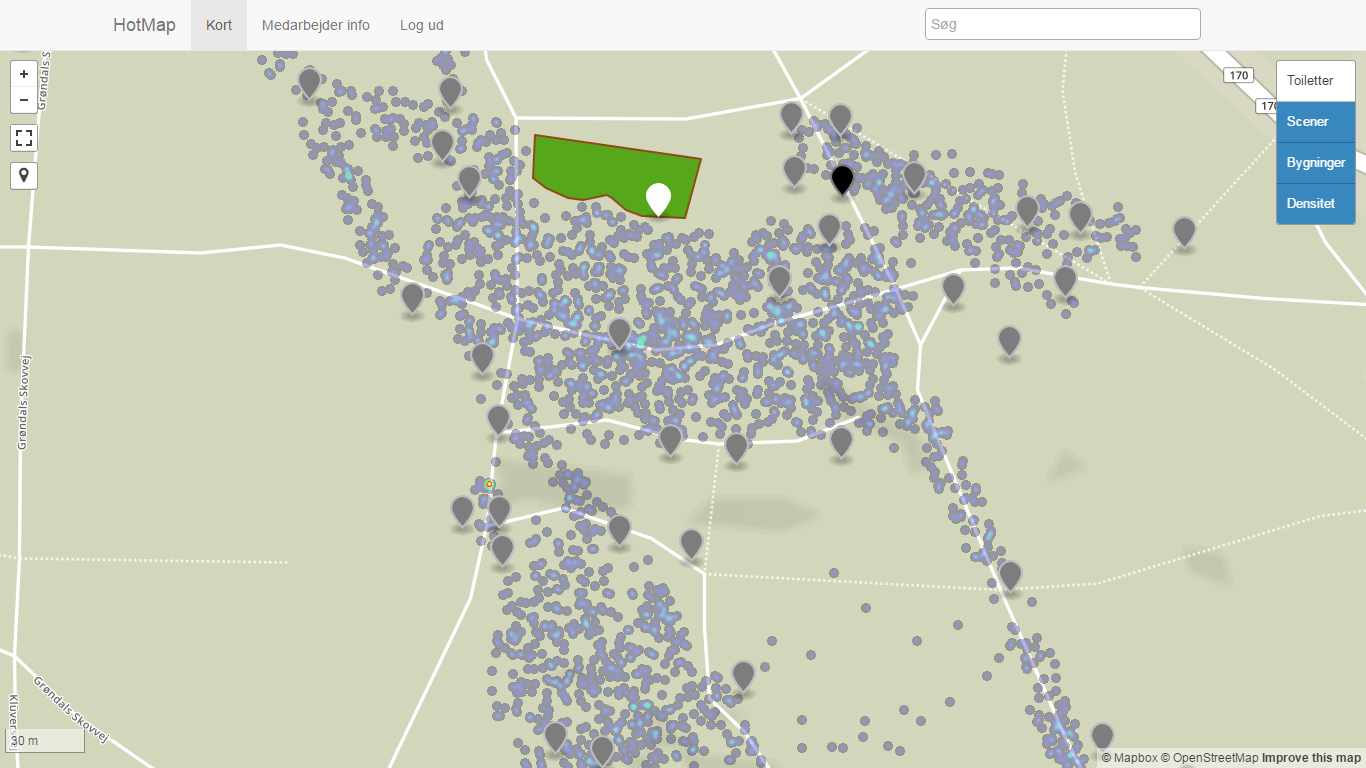
\includegraphics[width=\textwidth]{gui_desktop.png}
\caption{Screenshot of the application on a desktop computer}
\label{desktopscreenshot}
\end{figure}

\begin{figure}
    \centering
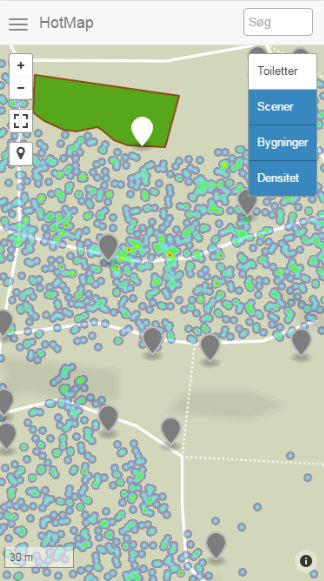
\includegraphics[width=\textwidth/3]{gui_phone.png}
\caption{Screenshot of the application on a smartphone}
\label{phonescreenshot}
\end{figure}
